\section{Web 2.0 - Abschlussarbeiten-DB}
Im Rahmen dieses Projektes ist ein relationales Schema und eine Menge an Datens\"atzen gegeben. Ziel ist es, dieses in eine NoSQL Lösung zu übertragen und die Datens\"atze in der Datenbank zu persistieren.

\subsection{Das semantische Schema}
In der Abbildung \ref{fig:schema1} ist das Schema der Datenbank zu sehen, die in den g\"angigen NoSQL Techniken umgesetzt werden soll. Eine Abschlussarbeit wird von einem "'Student"' oder einem "'Trainee"' geschrieben. Sowohl der "'Student"', als auch der "'Trainee"', als auch der "'Examiner"', als auch der "'Supervisor"' sind Unterklassen der Klasse "'Human"'. In Auftrag gegeben wird die Arbeit von einer "'Organisation"', die eine "'University"' oder eine "'Company"' sein kann. Die Arbeit wird eventuell von einer Menge von "'First\_Examiner"' und einer Menge von "'Second\_Examiner"' begutachtet, wenn es zu einem "'Degree"' f\"uhrt. Das mit dem "'Degree\_Topic"' verbundene "'Degree"' hat einen Titel. Das "'Topic"' kann in einer "'Topic\_Category"' liegen, in der gegebenenfalls auch der "'examiner"' oder die "'Company"' liegen. Dies bedeutet, die zentrale Klasse ist das "'Topic"', dass entweder ein "'Degree\_Topic"' oder ein "'Trainee\_Topic"' ist. Hierbei ist das "'Degree\_Topic"' wiederum entweder die "'Bachelor\_Thesis"' oder die "'Master\_Thesis"'.\\

Das Schema deutet also an, dass ein Mensch, der eine Abschlussarbeit schreibt, entweder ein Auszubildender oder ein Student ist. Diese Abschlussarbeit schreibende Person schreibt die Arbeit entweder im Rahmen einer Ausbildung oder im Rahmen eines Studiums, der mit einem Abschluss ("'Degree"') belegt ist. 

Insgesamt sind 27 Klassen gegeben, auf denen 36 Attribute verteilt sind.\\

\begin{figure}[H]
	\centering
	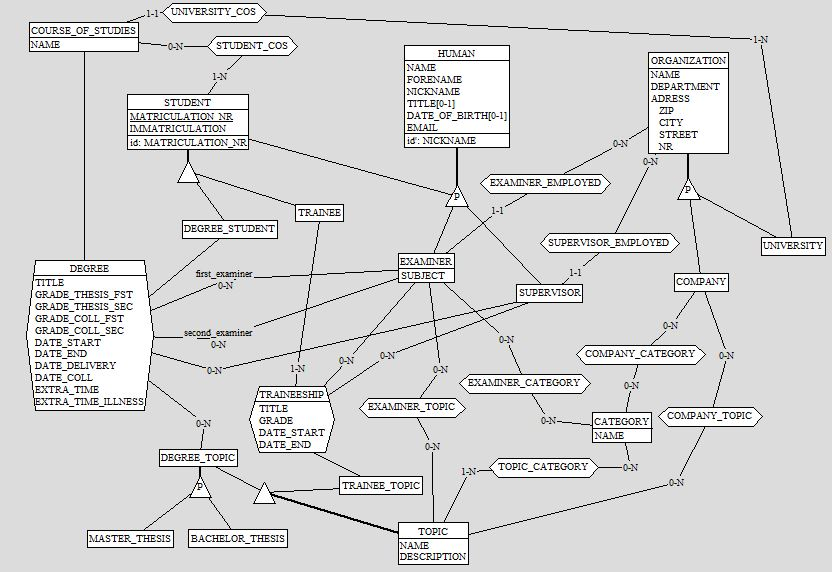
\includegraphics[scale=0.6]{images/01abschlussarbeitendbschema.jpg} 
	\caption{AbschlussarbeitenDB Schema}\label{fig:schema1}
\end{figure}

\subsection{Die Datenbestände}
Wie in Abbildung \ref{fig:schema2} zu sehen gibt es insgesamt 21 Spalten. Diese 21 Spalten repräsentieren 21 Attribute, die eine deutliche Differenz zu den 36 Attributen des Schemas darstellen. Dies bedeutet, in den Datenbeständen sind weniger ausführliche Daten gegeben, als eigentlich durch das Schema vorgegeben. \\

\begin{figure}[H]
	\centering
	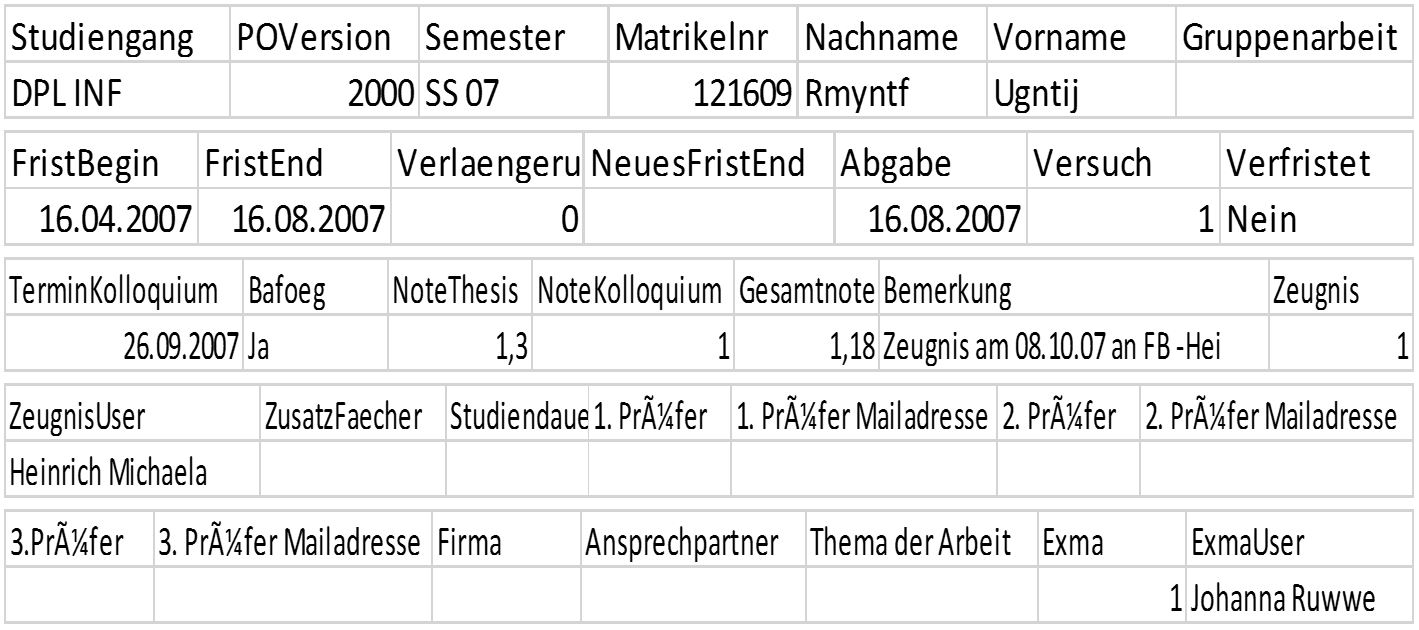
\includegraphics[scale=0.3]{images/01beispieldatensatzcsv.jpg} 
	\caption{Beispiel-Datensatz}\label{fig:schema2}
\end{figure}
